As with any high-dimensional optimization problem, the fitter must be vigilant
against the overfitting of data. In practice, this requires:

parsimony with the number of parameters used in the model

common-sense checking "under the hood" of the optimization to verify that
parameter values make sense given the assumptions that undergird the model

understanding of what the value function is (that is, the function being
minimized/maximized) and whether it needs to be changed

cross-correlation between parameters to understand the relationship between
parameters and the effect that each has on predictions made using the model

TCS affected by HF parameters, spin orbit, imaginary above
RCS affected by imaginary above, HF parameters
ECS affected by HF parameters, spin orbit, imaginary above
APower affected by HF parameters, spin orbit,  imaginary above
Charge Density affected by HF parameters, imaginary below
Levels affected by HF parameters, spin orbit,
Spectral functions affected by HF parameters, imaginary below
RMSRadii affected by HF parameters, imaginary below

\subsection{Fitting procedure}
The powell method, outlined in Numerical Recipes in C \cite{NumericalRecipes},
was used to minimize the RMS difference between experimental data points and the
values calculated by the DOM. A weighting scheme was assigned to the data points
according to their importance, guiding the fit to reproduce the most essential
data points. From fit to fit, the weighting scheme was adjusted as necessary to
escape local minima in the multidimensional fit.

\begin{figure}
\begin{center}
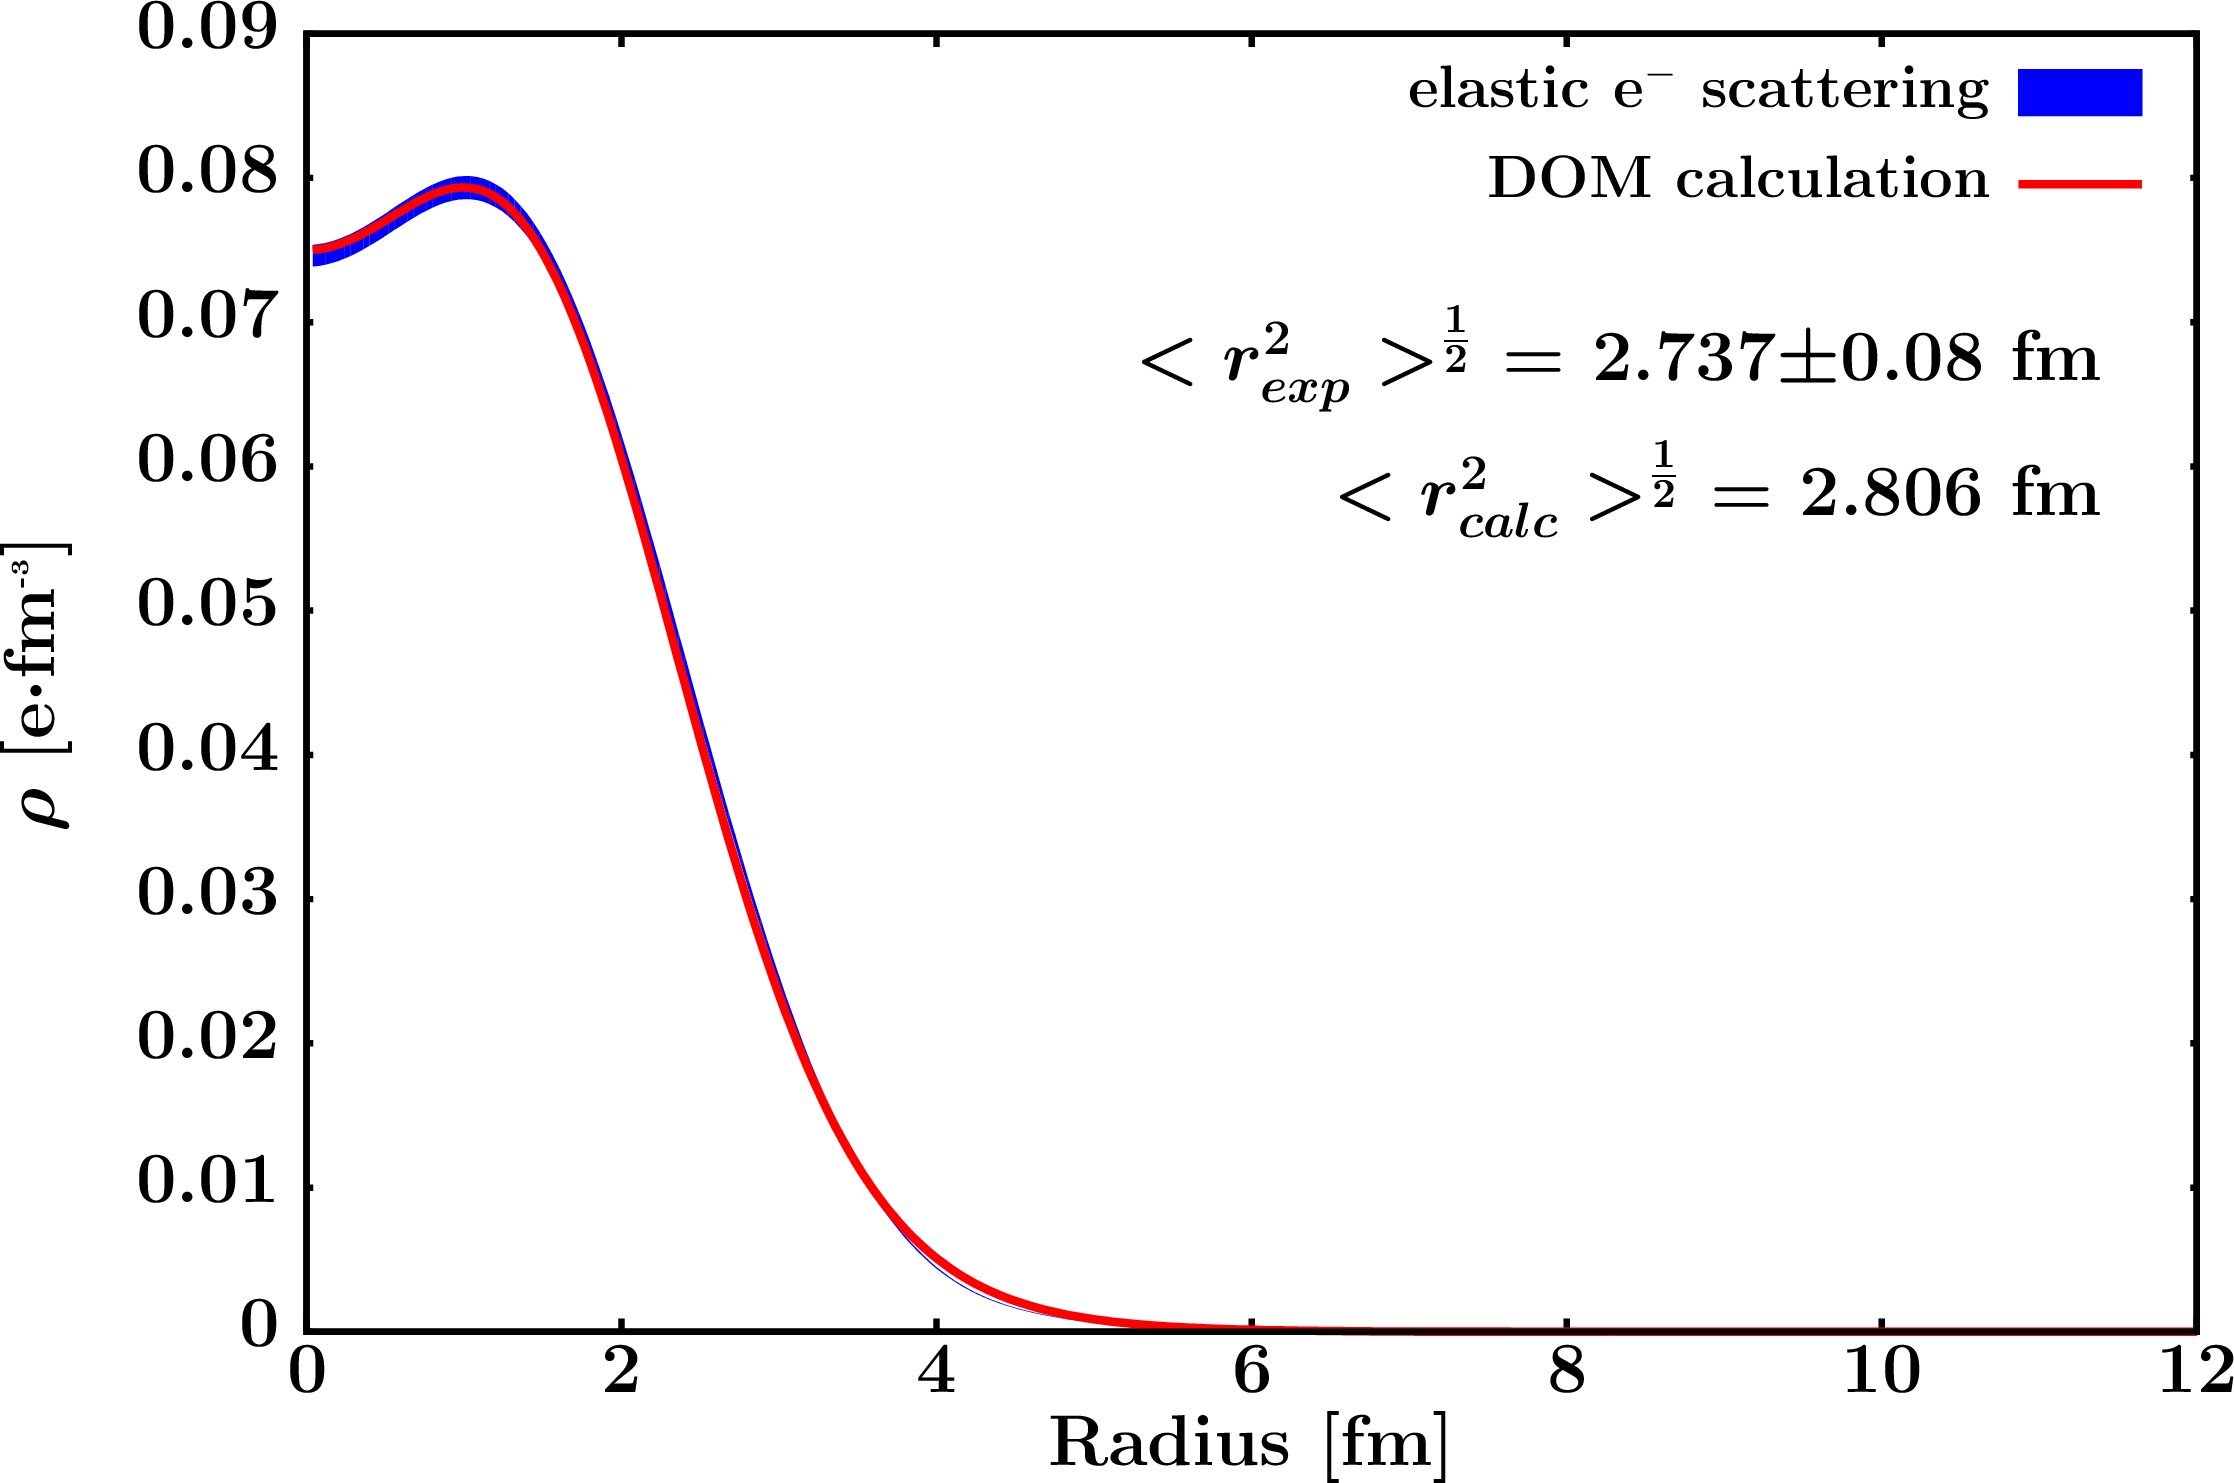
\includegraphics[width = 0.9\textwidth]{figures/o16_chargeDensity.png}
\caption{DOM fit of $^{16}O$ charge density}
\label{o16ChargeDensity}
\end{center}
\end{figure}

\begin{figure}
\begin{center}
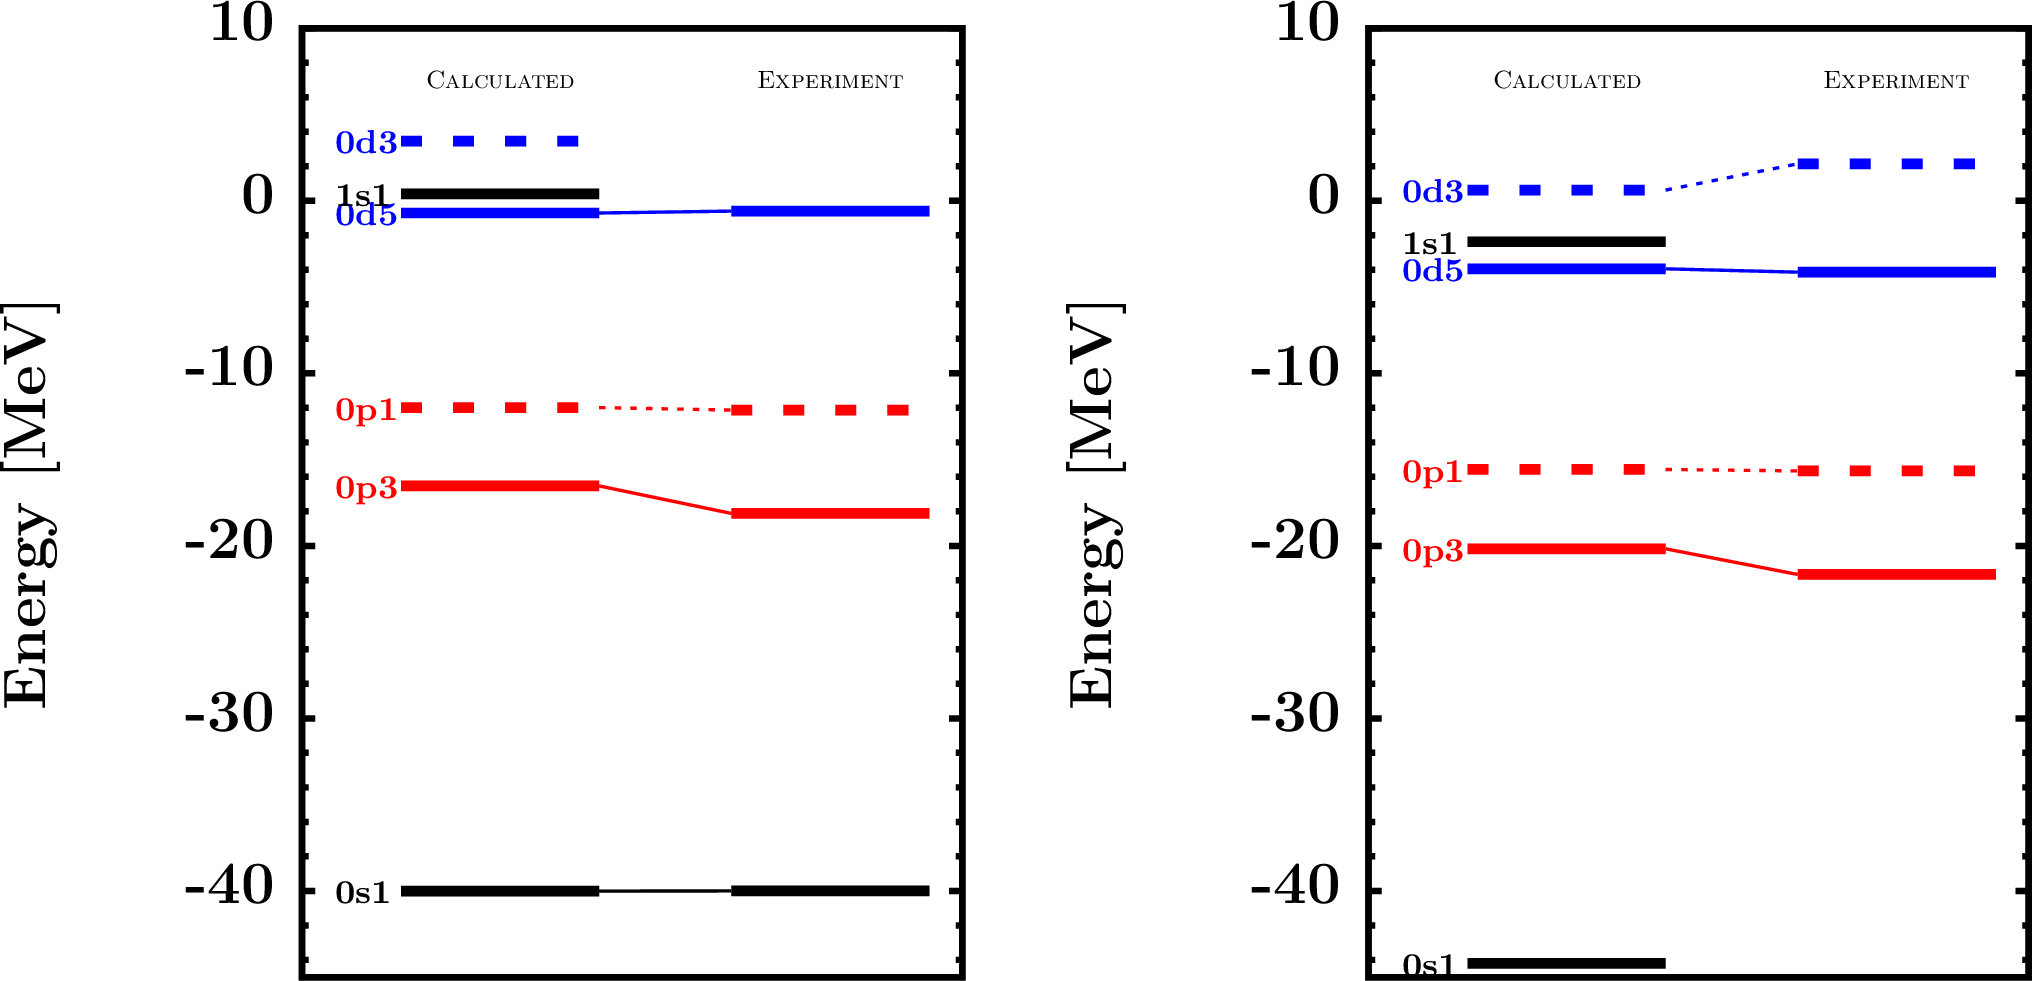
\includegraphics[width = 0.9\textwidth]{figures/o16_SPLevels.png}
\caption{DOM fit of $^{16}O$ single-particle levels}
\label{o16SPLevels}
\end{center}
\end{figure}

\begin{figure}
\begin{center}
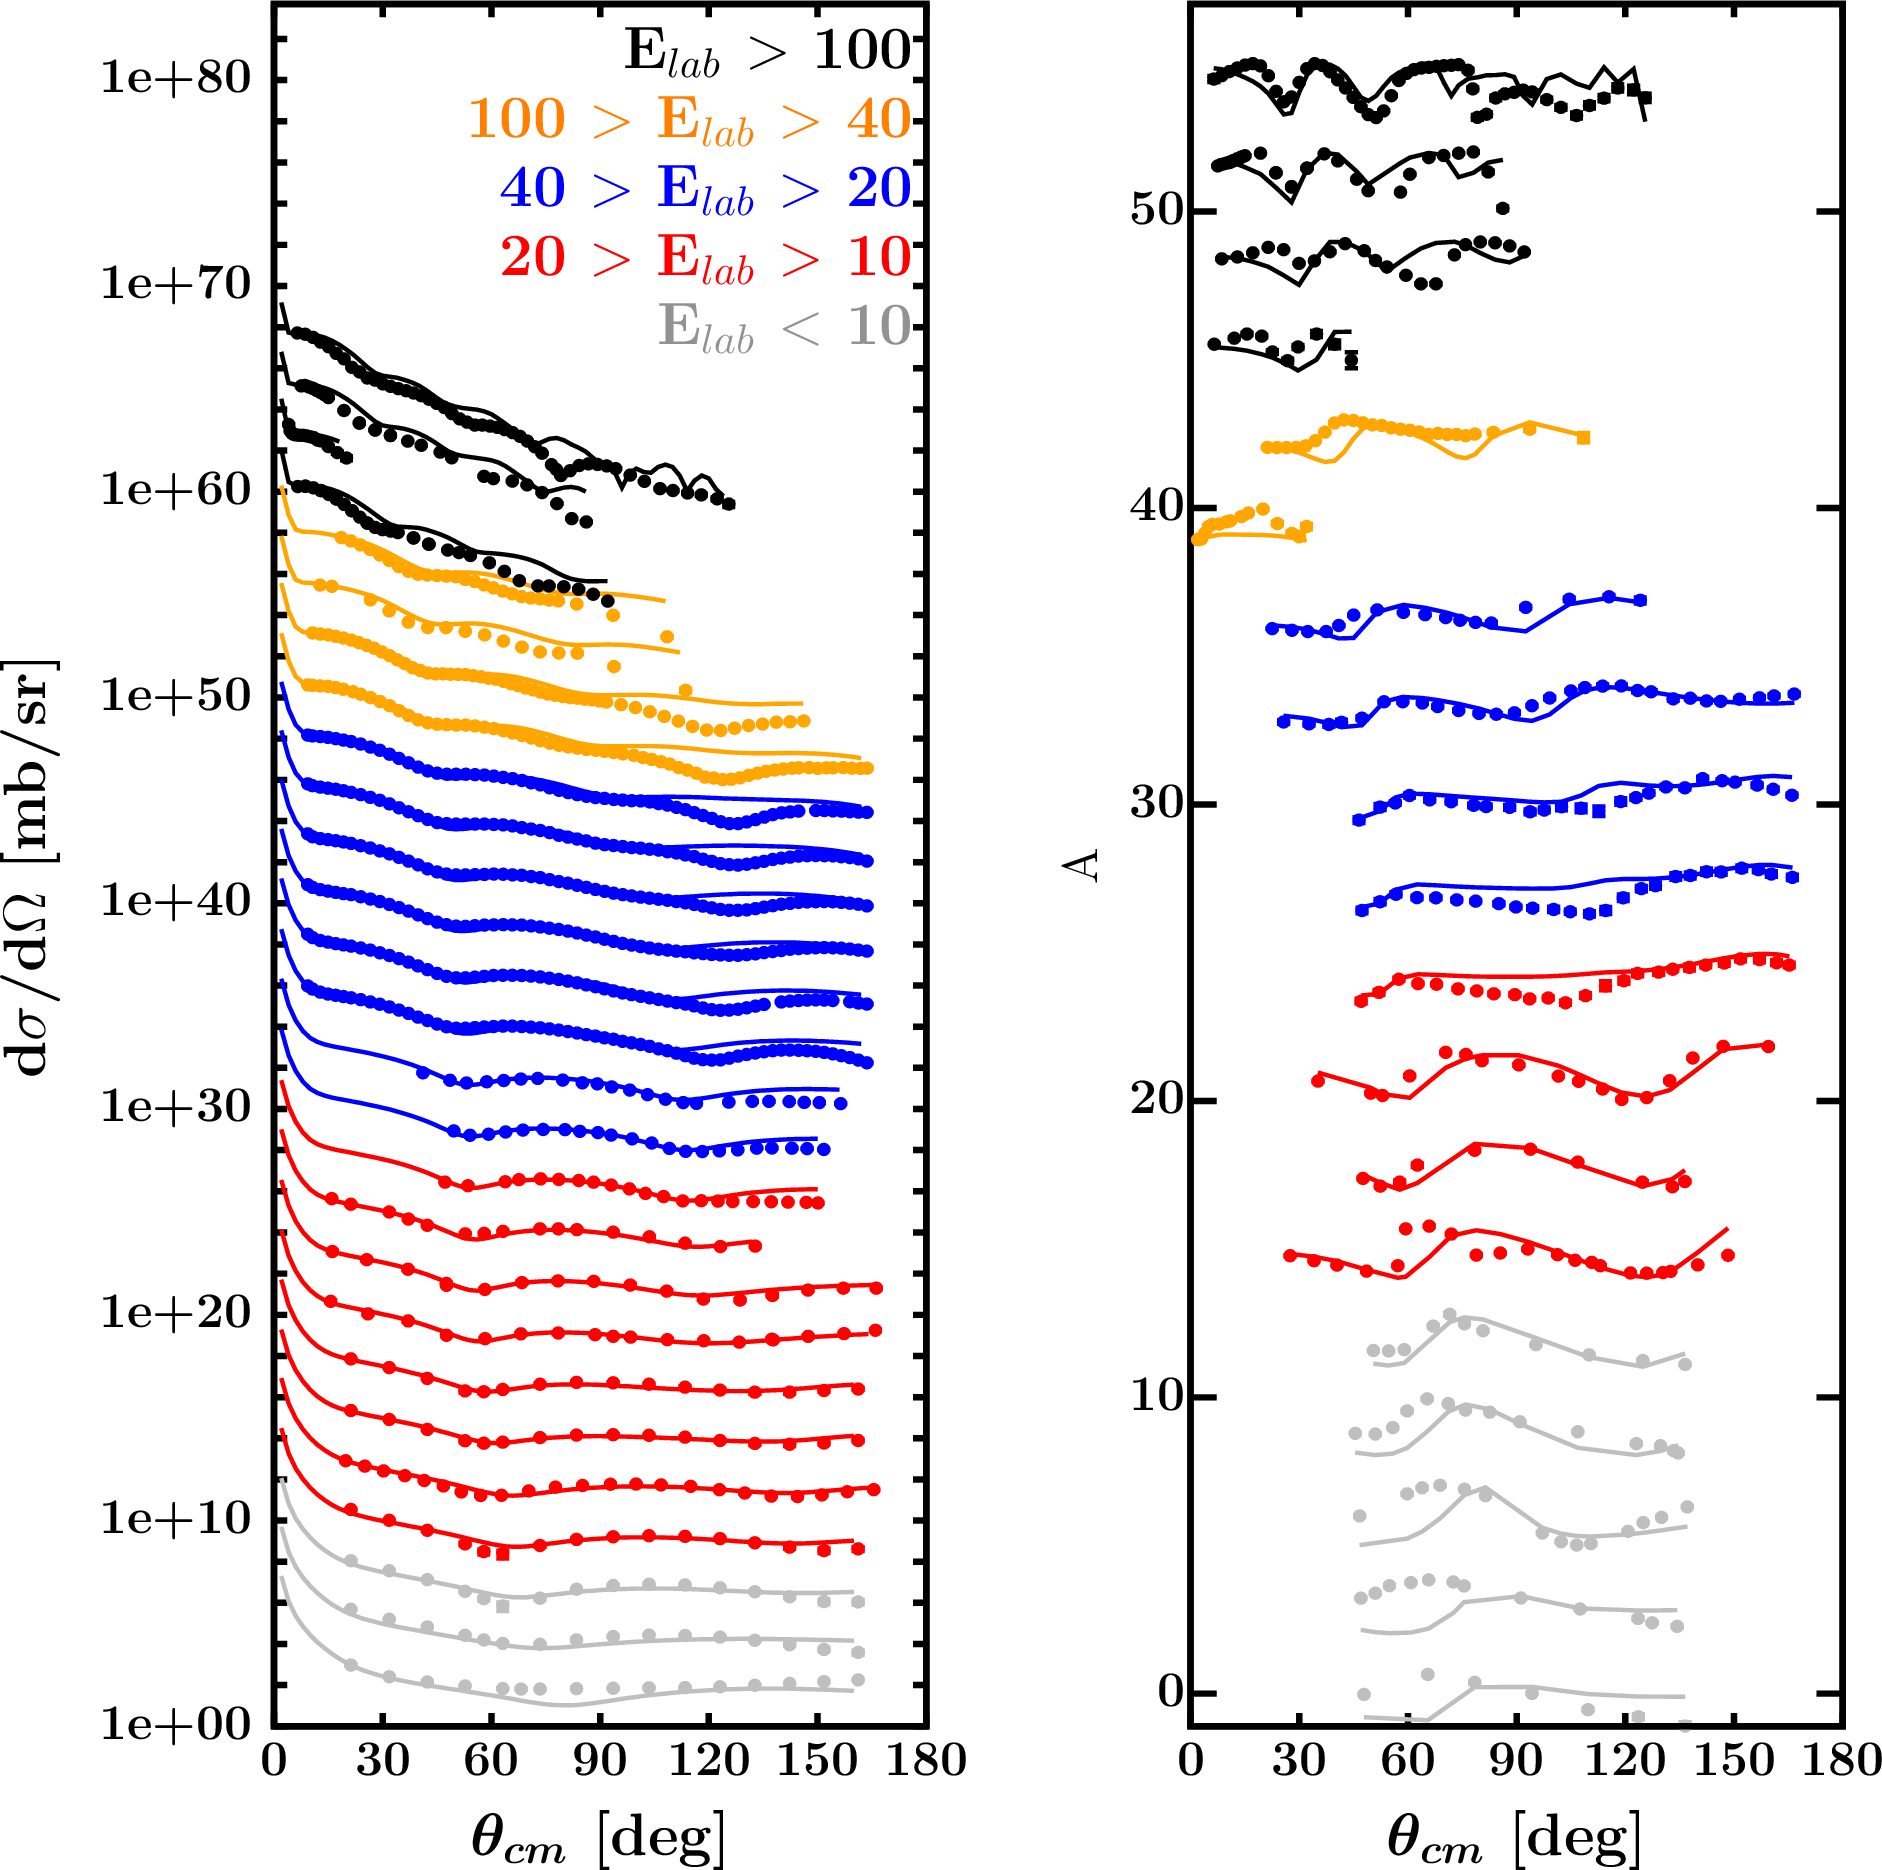
\includegraphics[width = 0.9\textwidth]{figures/o16_protonElastic.png}
\caption{DOM fit of $^{16}O$ proton elastic scattering data}
\label{o16ProtonElastic}
\end{center}
\end{figure}

\begin{figure}
\begin{center}
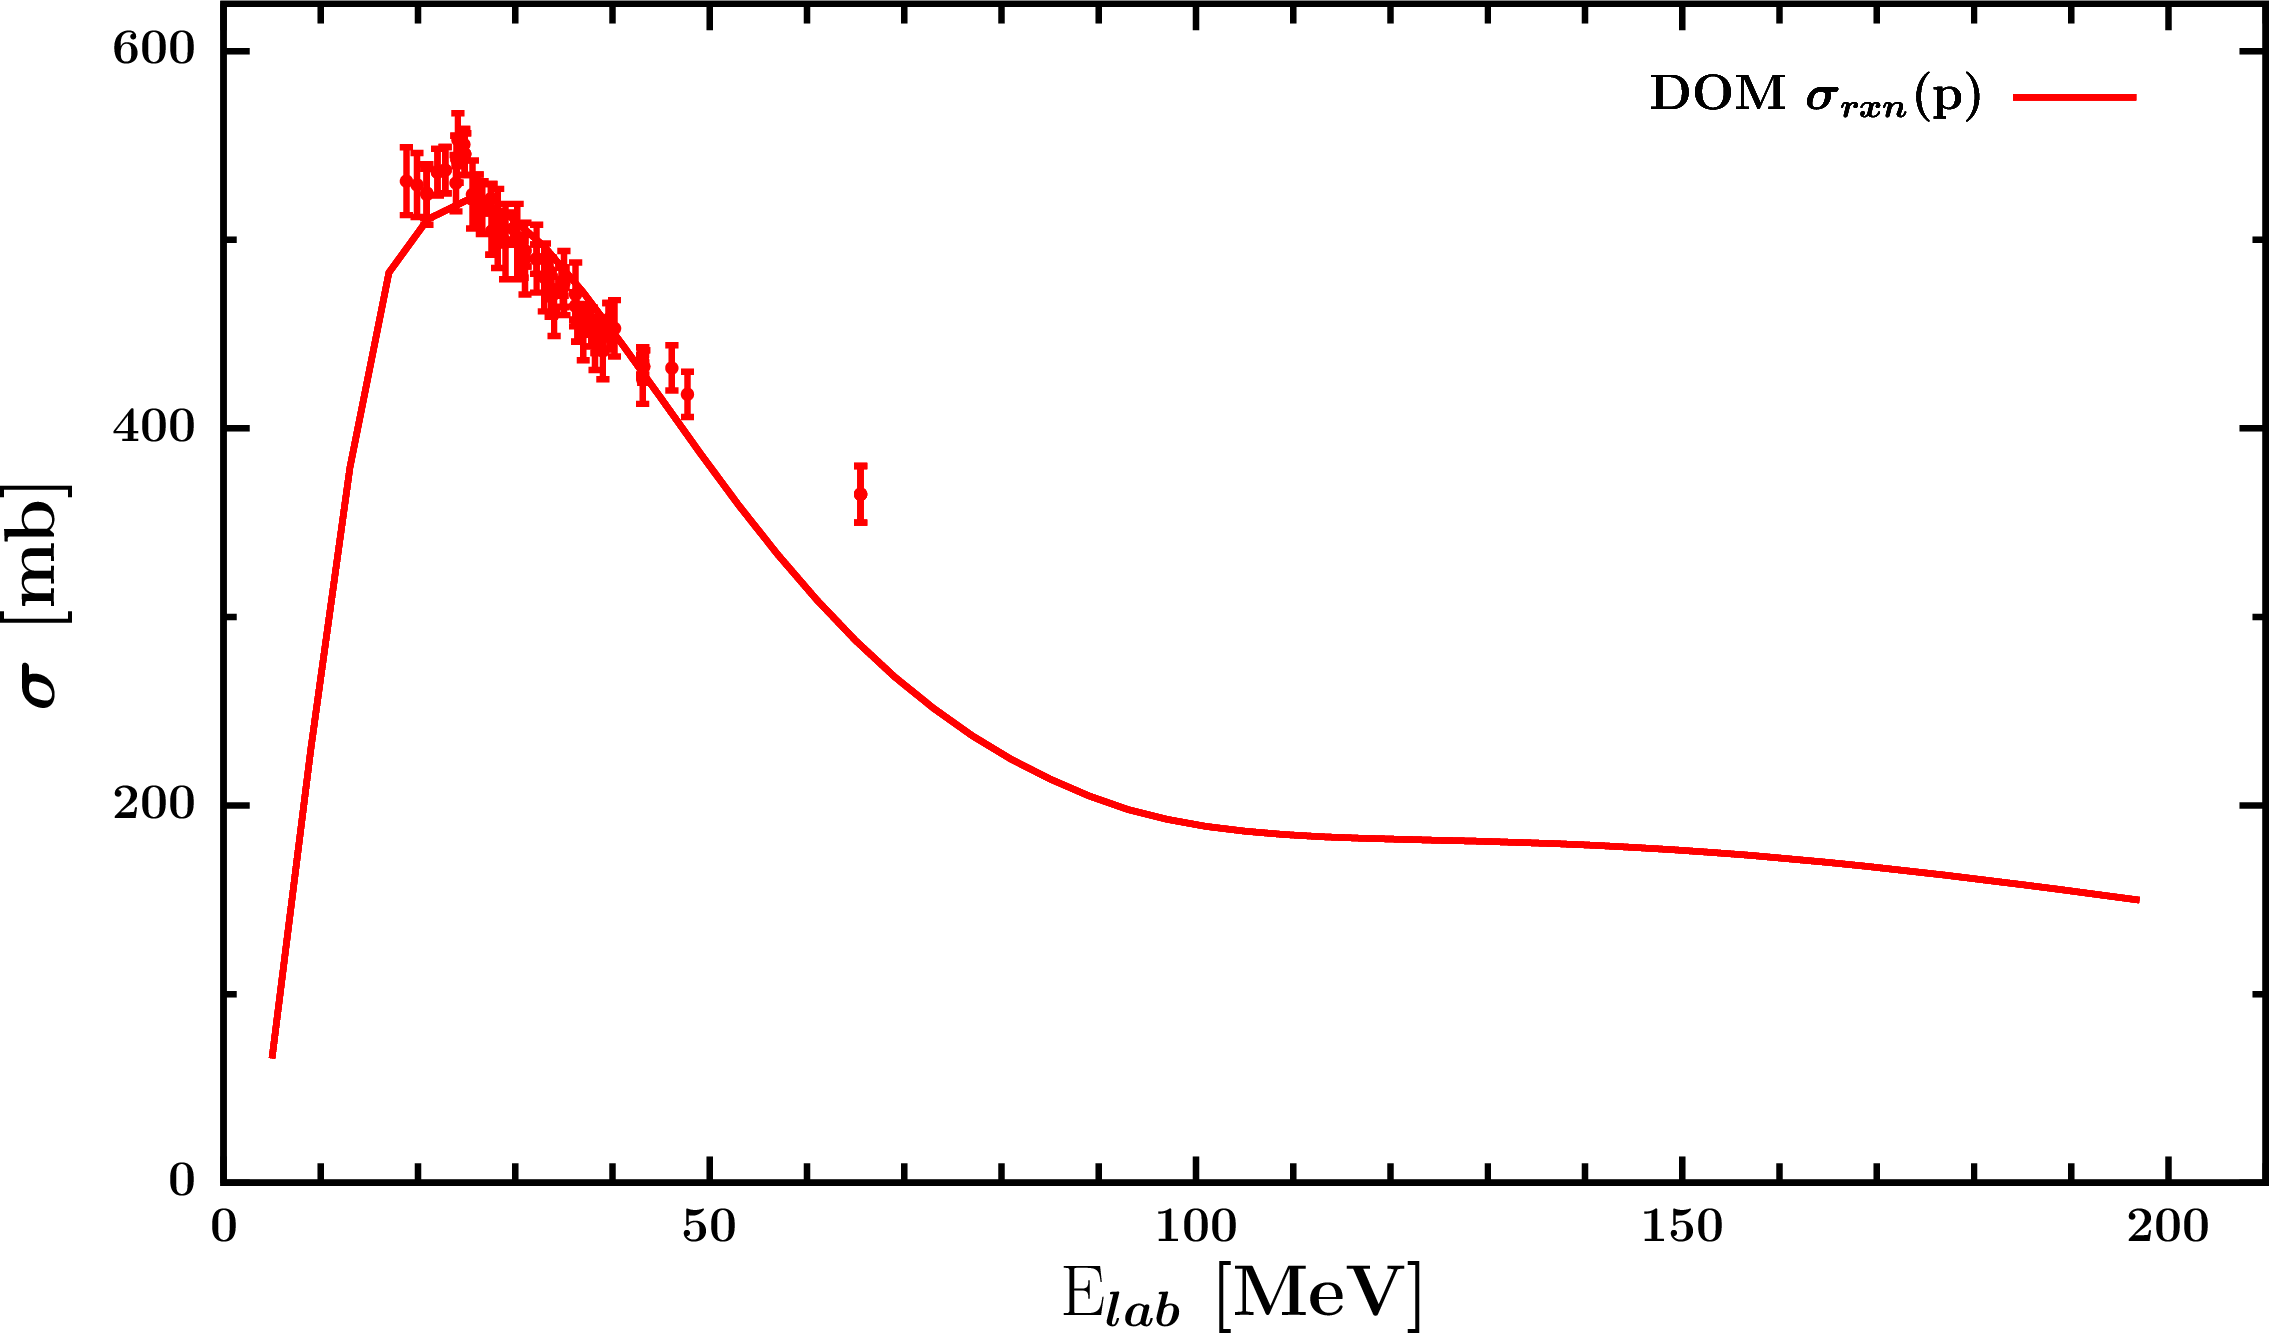
\includegraphics[width = 0.9\textwidth]{figures/o16_protonInelastic.png}
\caption{DOM fit of $^{16}O$ proton inelastic scattering data}
\label{o16ProtonInelastic}
\end{center}
\end{figure}

\begin{figure}
\begin{center}
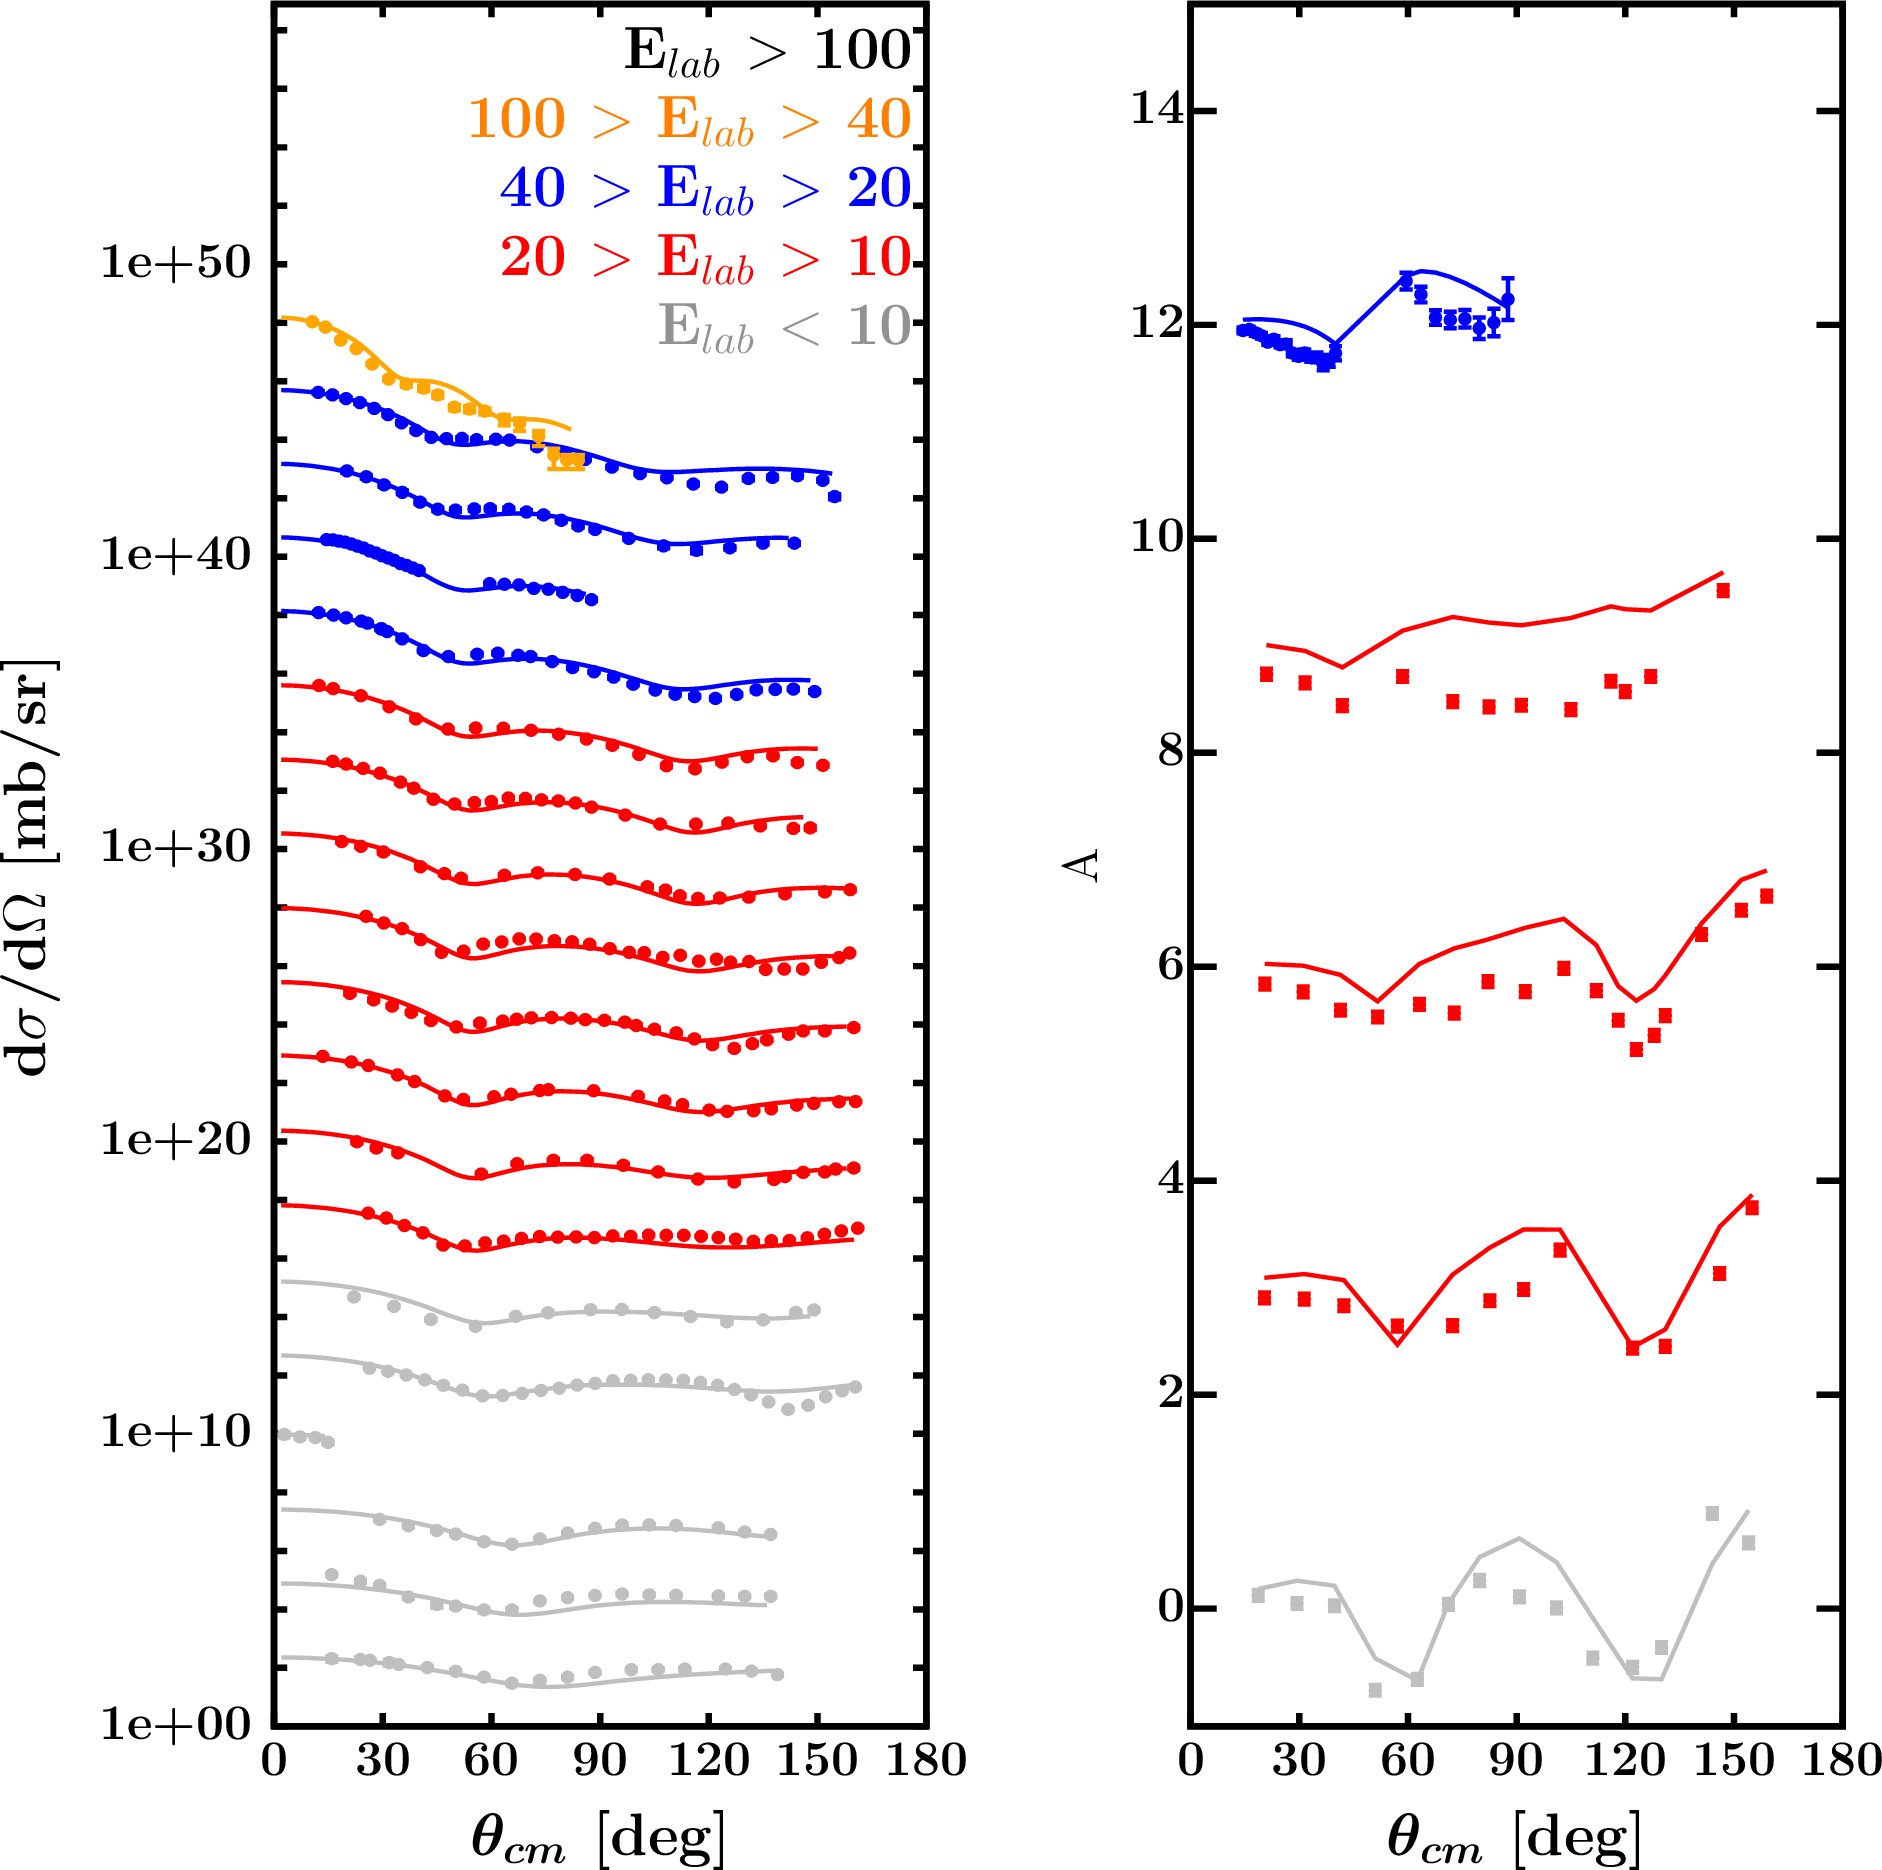
\includegraphics[width = 0.9\textwidth]{figures/o16_neutronElastic.png}
\caption{DOM fit of $^{16}O$ neutron elastic scattering data}
\label{o16NeutronElastic}
\end{center}
\end{figure}

\begin{figure}
\begin{center}
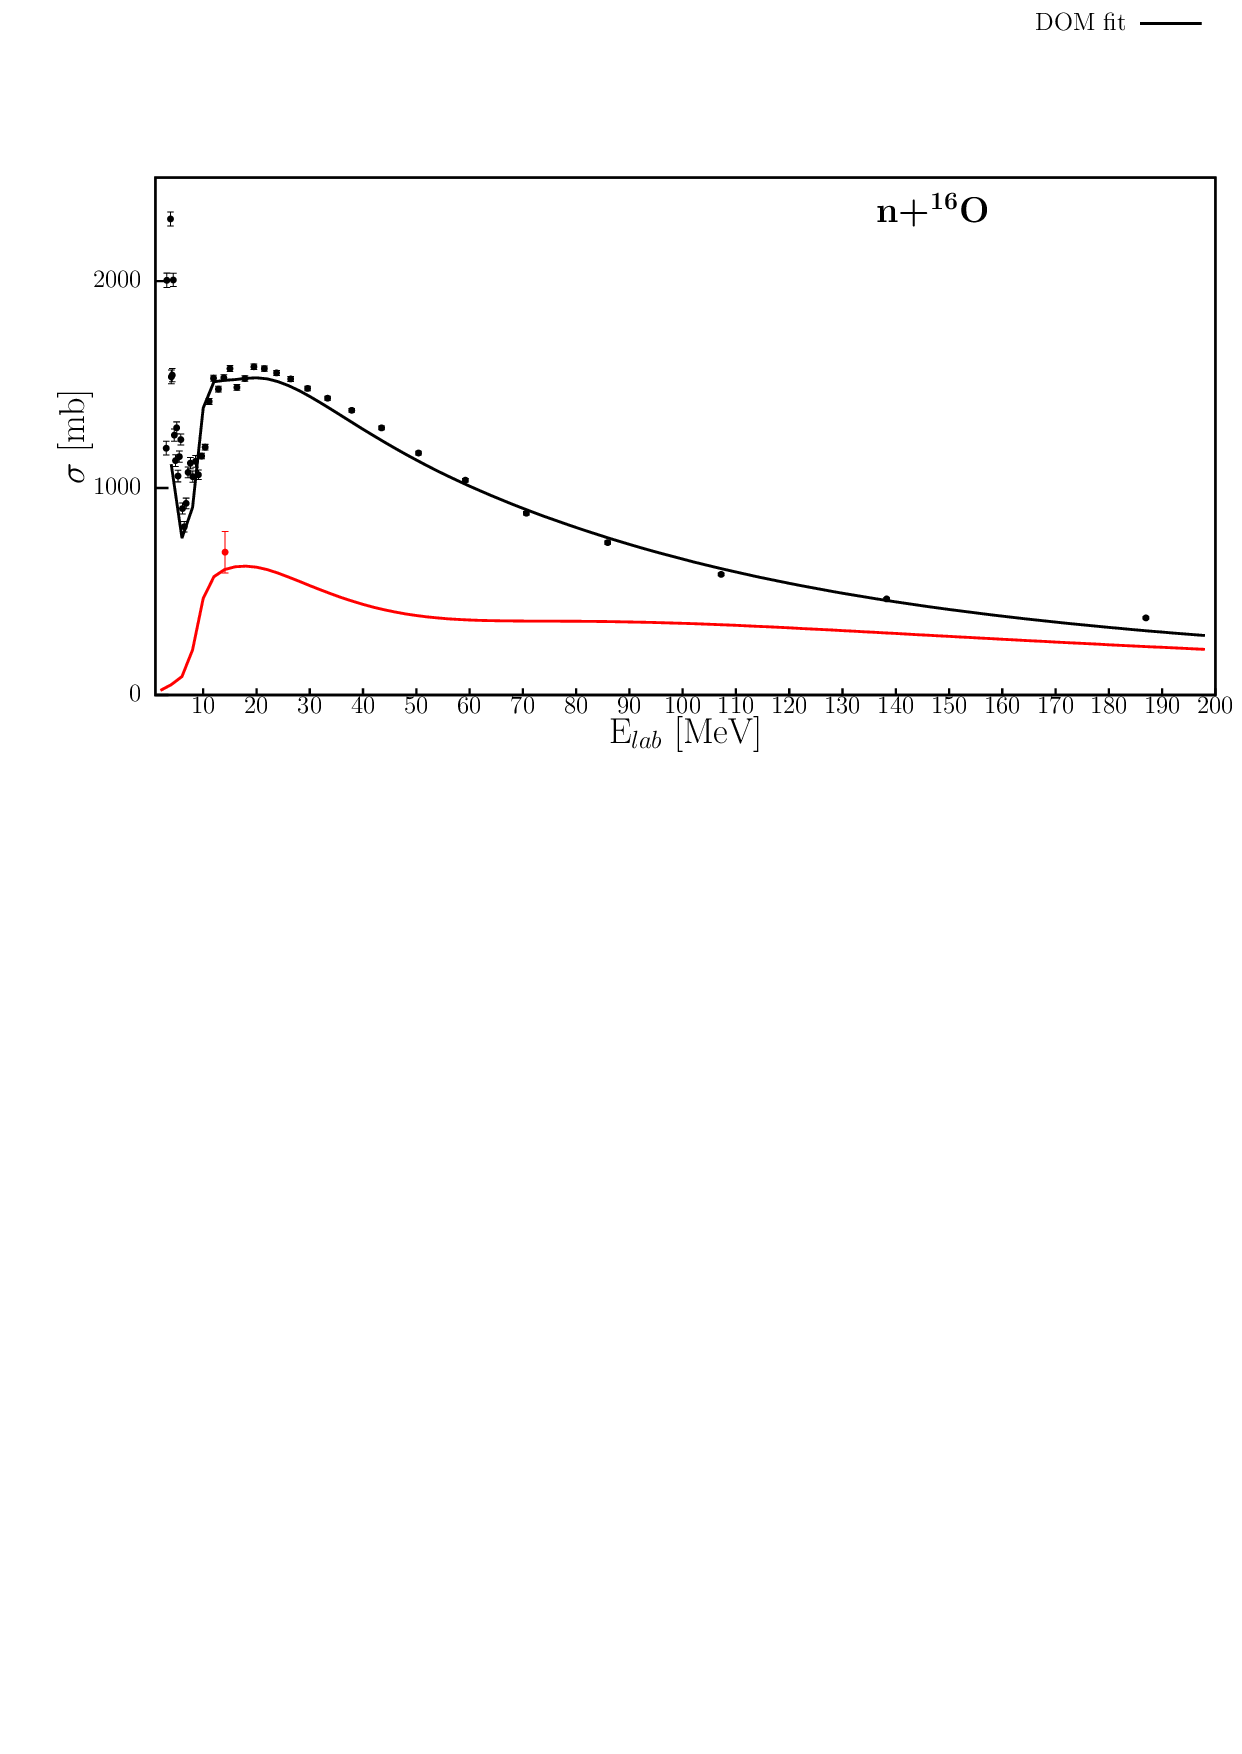
\includegraphics[width = 0.9\textwidth]{figures/o16_neutronInelastic.png}
\caption{DOM fit of $^{16}O$ neutron inelastic scattering data}
\label{o16NeutronInelastic}
\end{center}
\end{figure}

\begin{figure}
\begin{center}
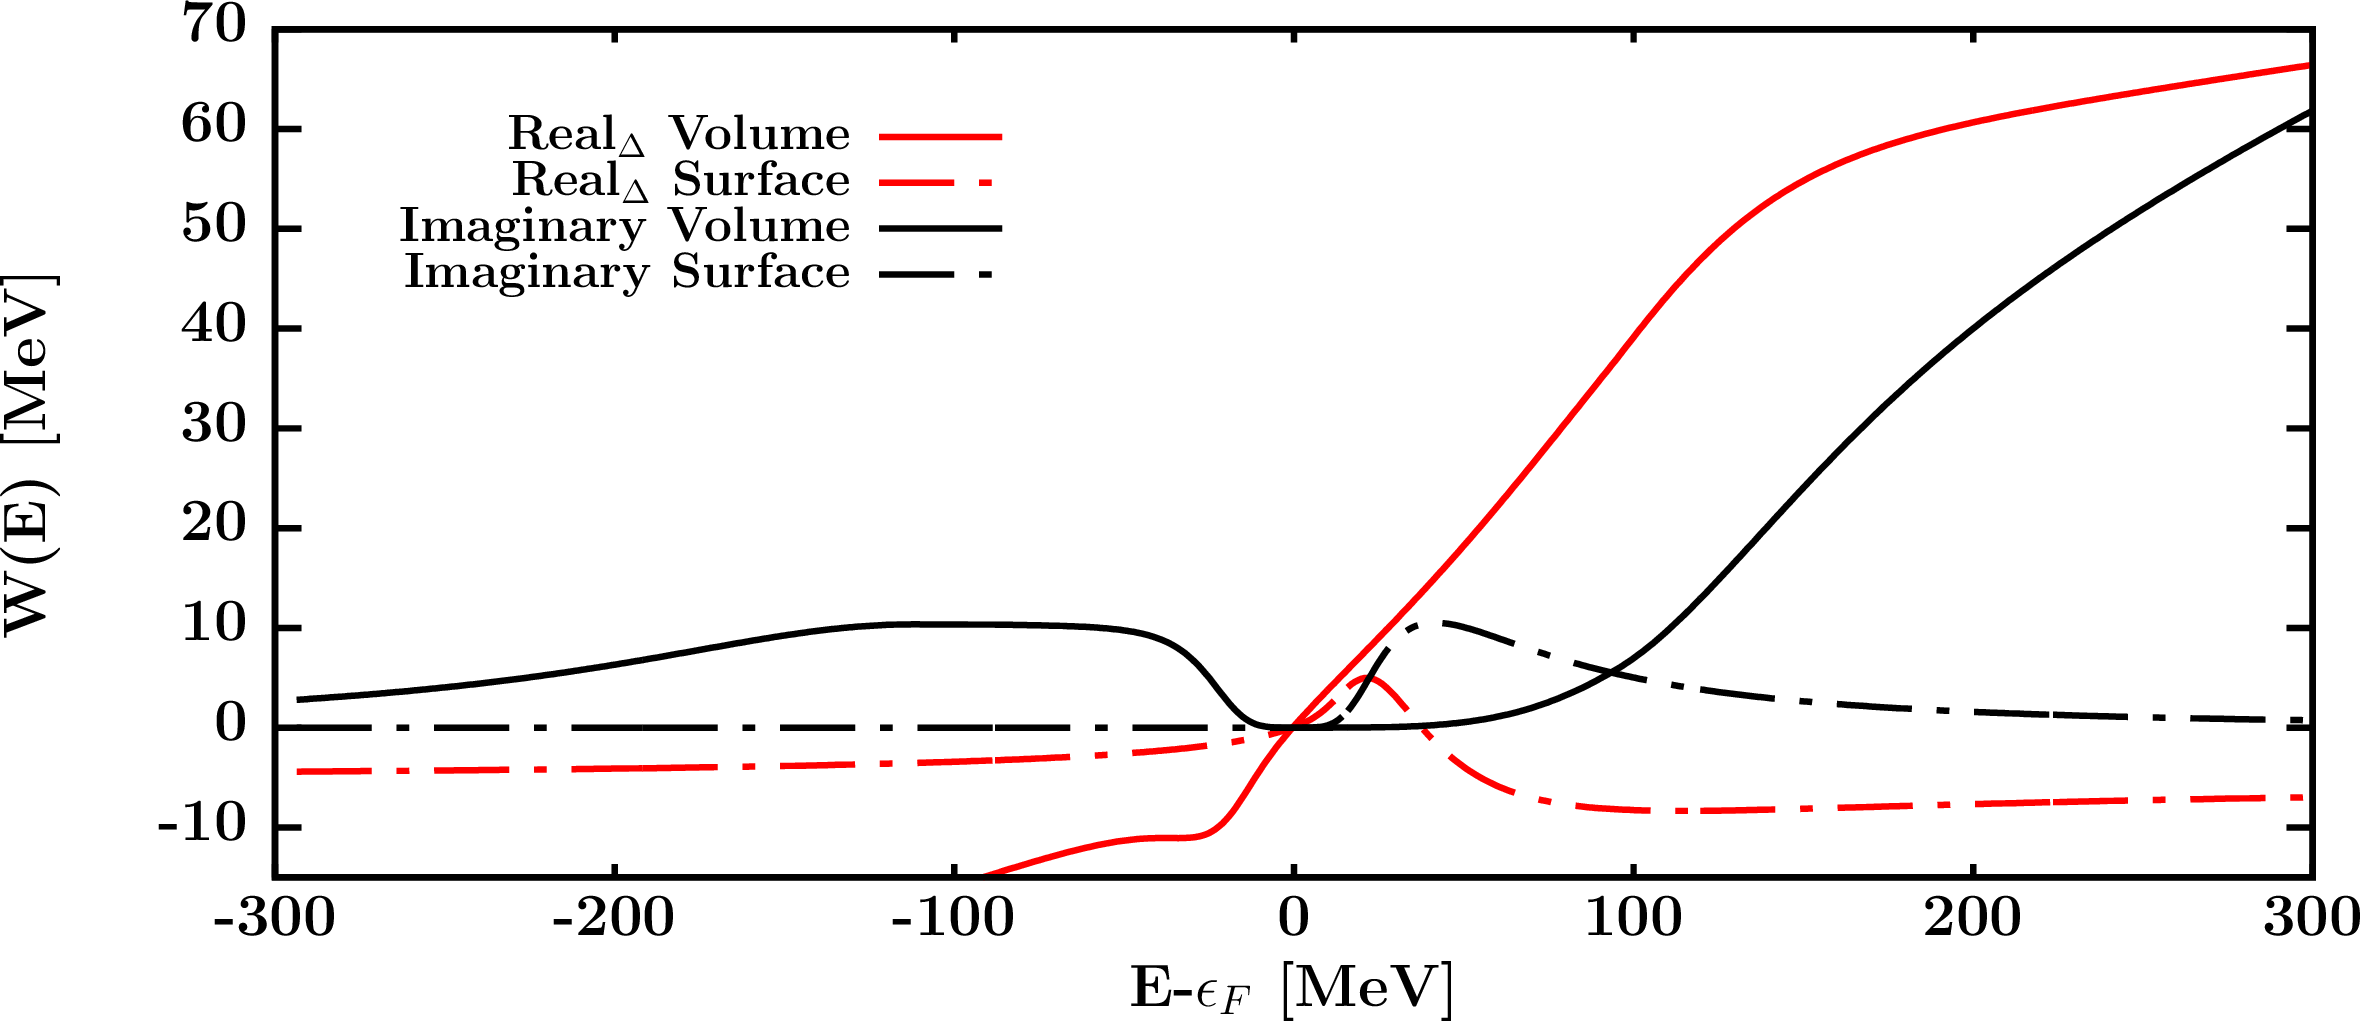
\includegraphics[width = 0.9\textwidth]{figures/o16_protonPotentials.png}
\caption{Visualization of DOM optical potential components for protons on
$^{16}O$}
\label{o16ProtonPotentials}
\end{center}
\end{figure}

\begin{figure}
\begin{center}
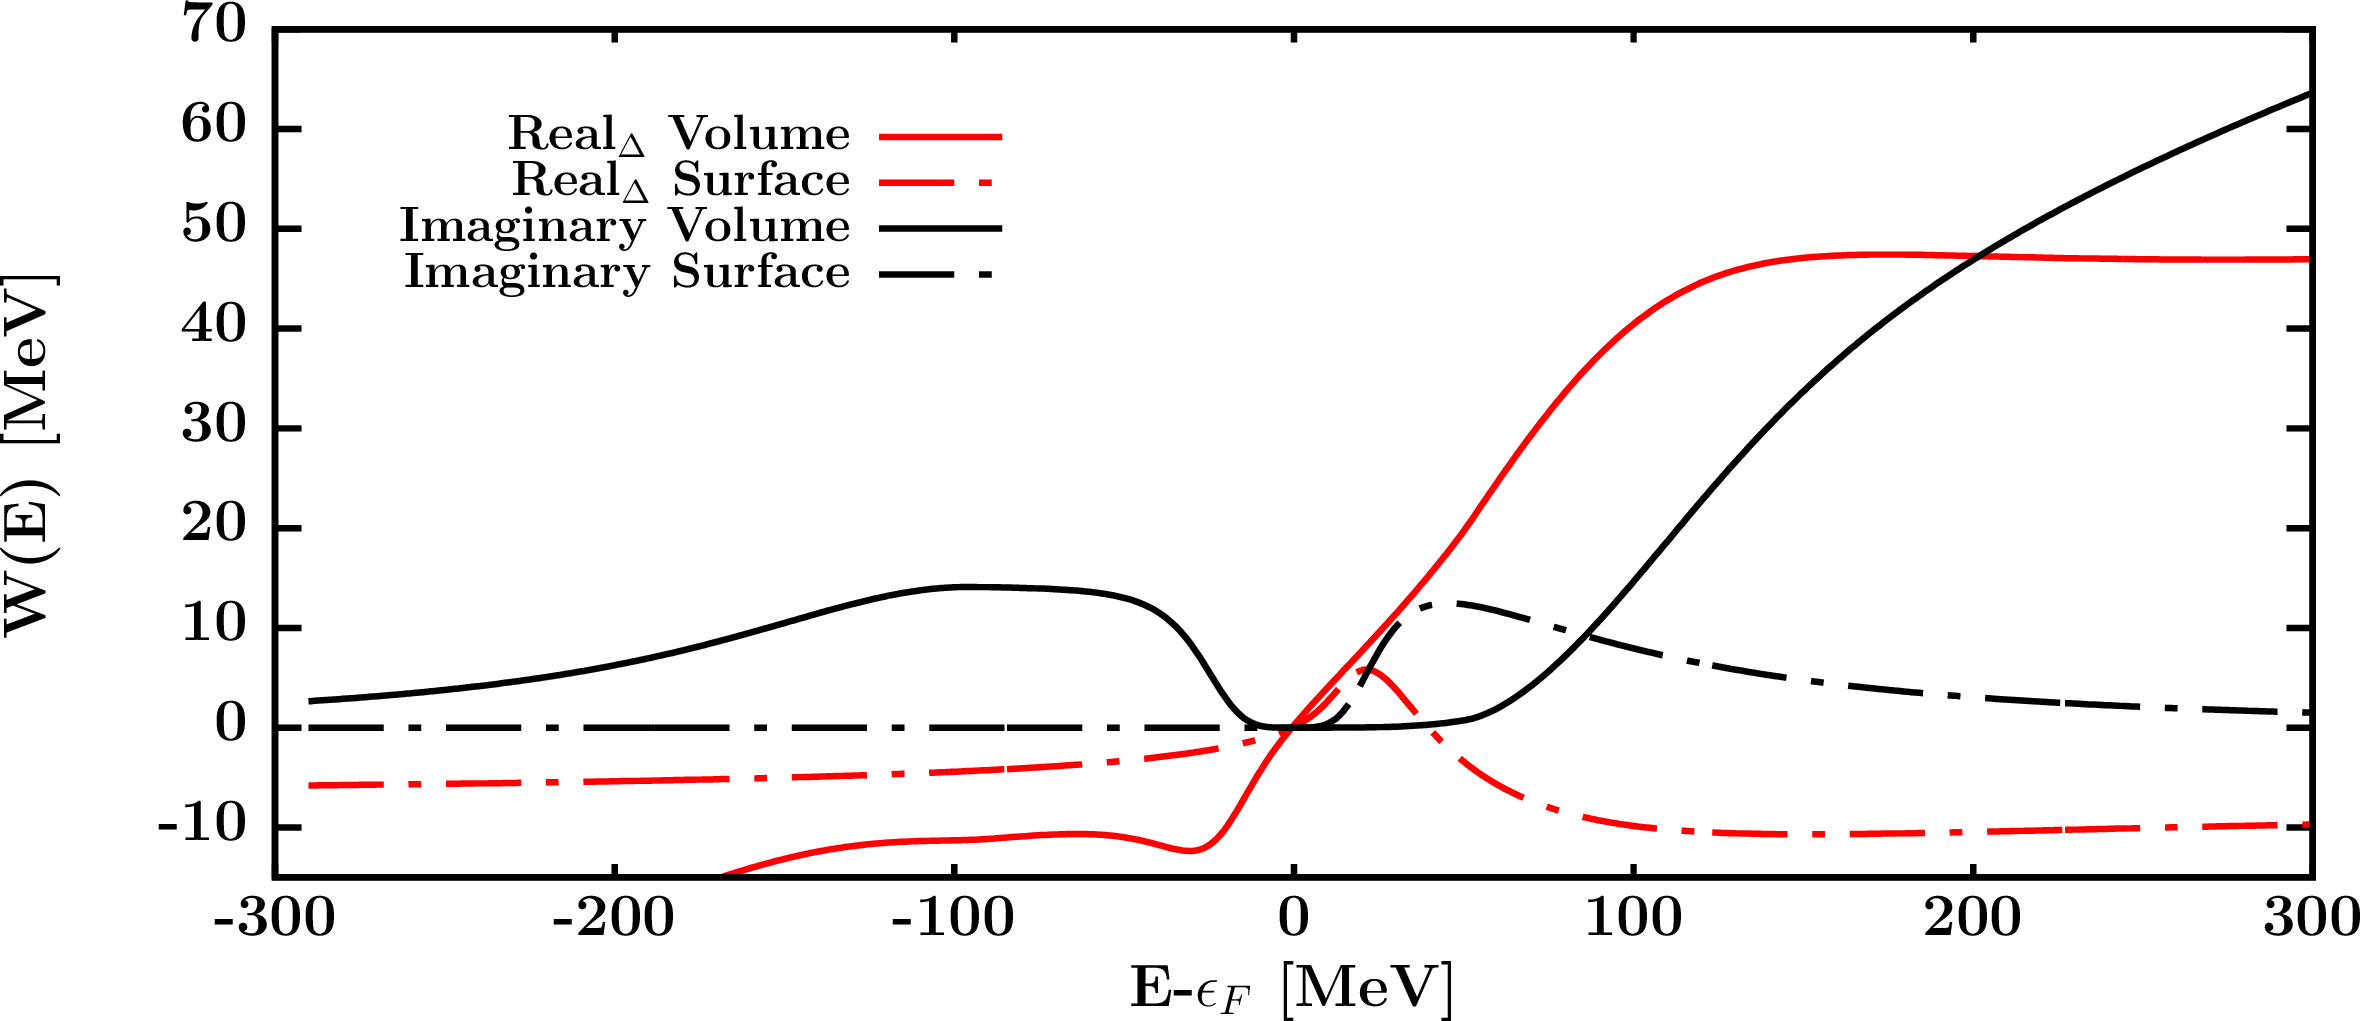
\includegraphics[width = 0.9\textwidth]{figures/o16_neutronPotentials.png}
\caption{Visualization of DOM optical potential components for neutrons on
$^{16}O$}
\label{o16NeutronPotentials}
\end{center}
\end{figure}

\begin{figure}
\begin{center}
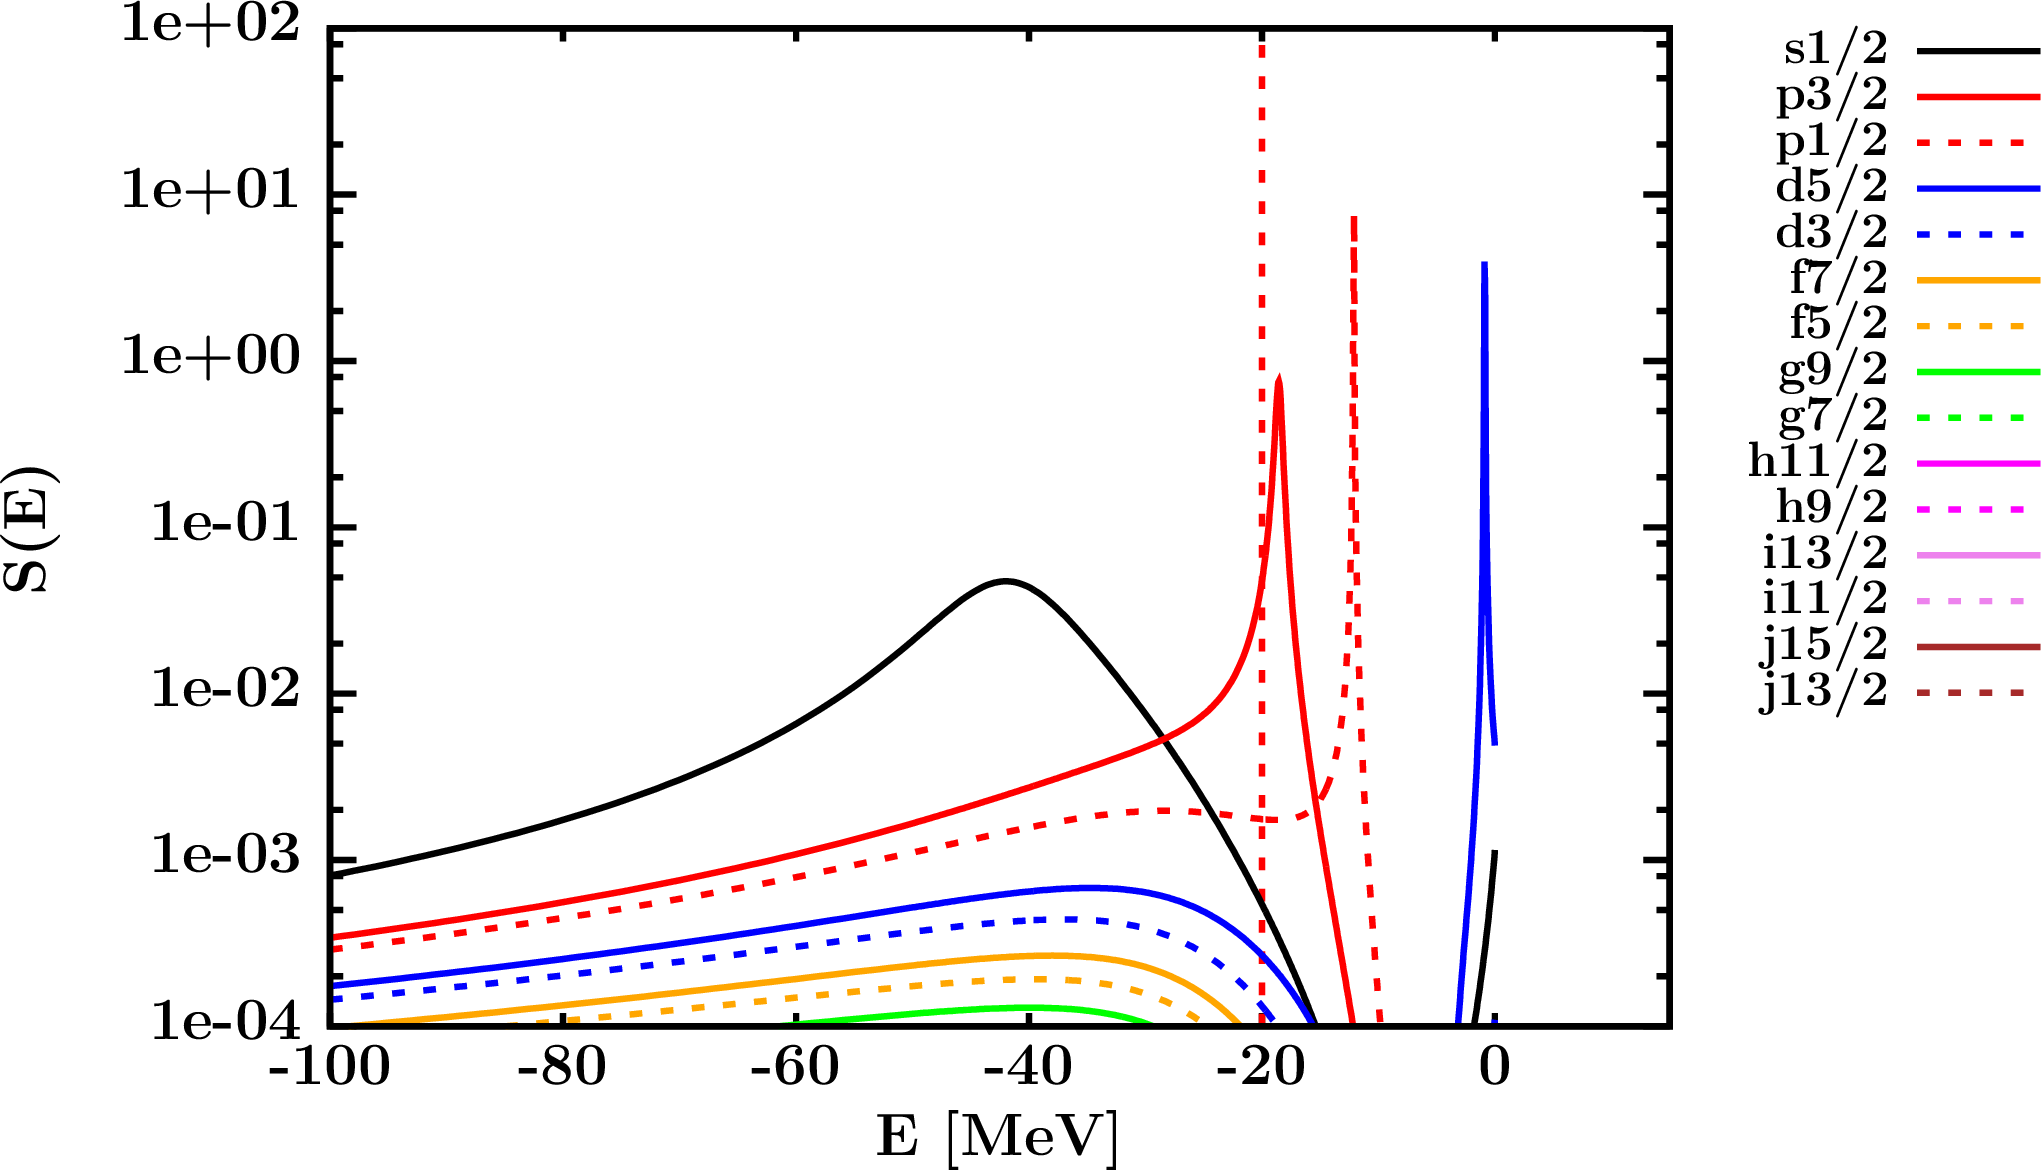
\includegraphics[width = 0.9\textwidth]{figures/o16_protonSpectralFunctions.png}
\caption{DOM calculation of $^{16}O$ proton spectral functions}
\label{o16ProtonSpectralFunctions}
\end{center}
\end{figure}


\begin{figure}
\begin{center}
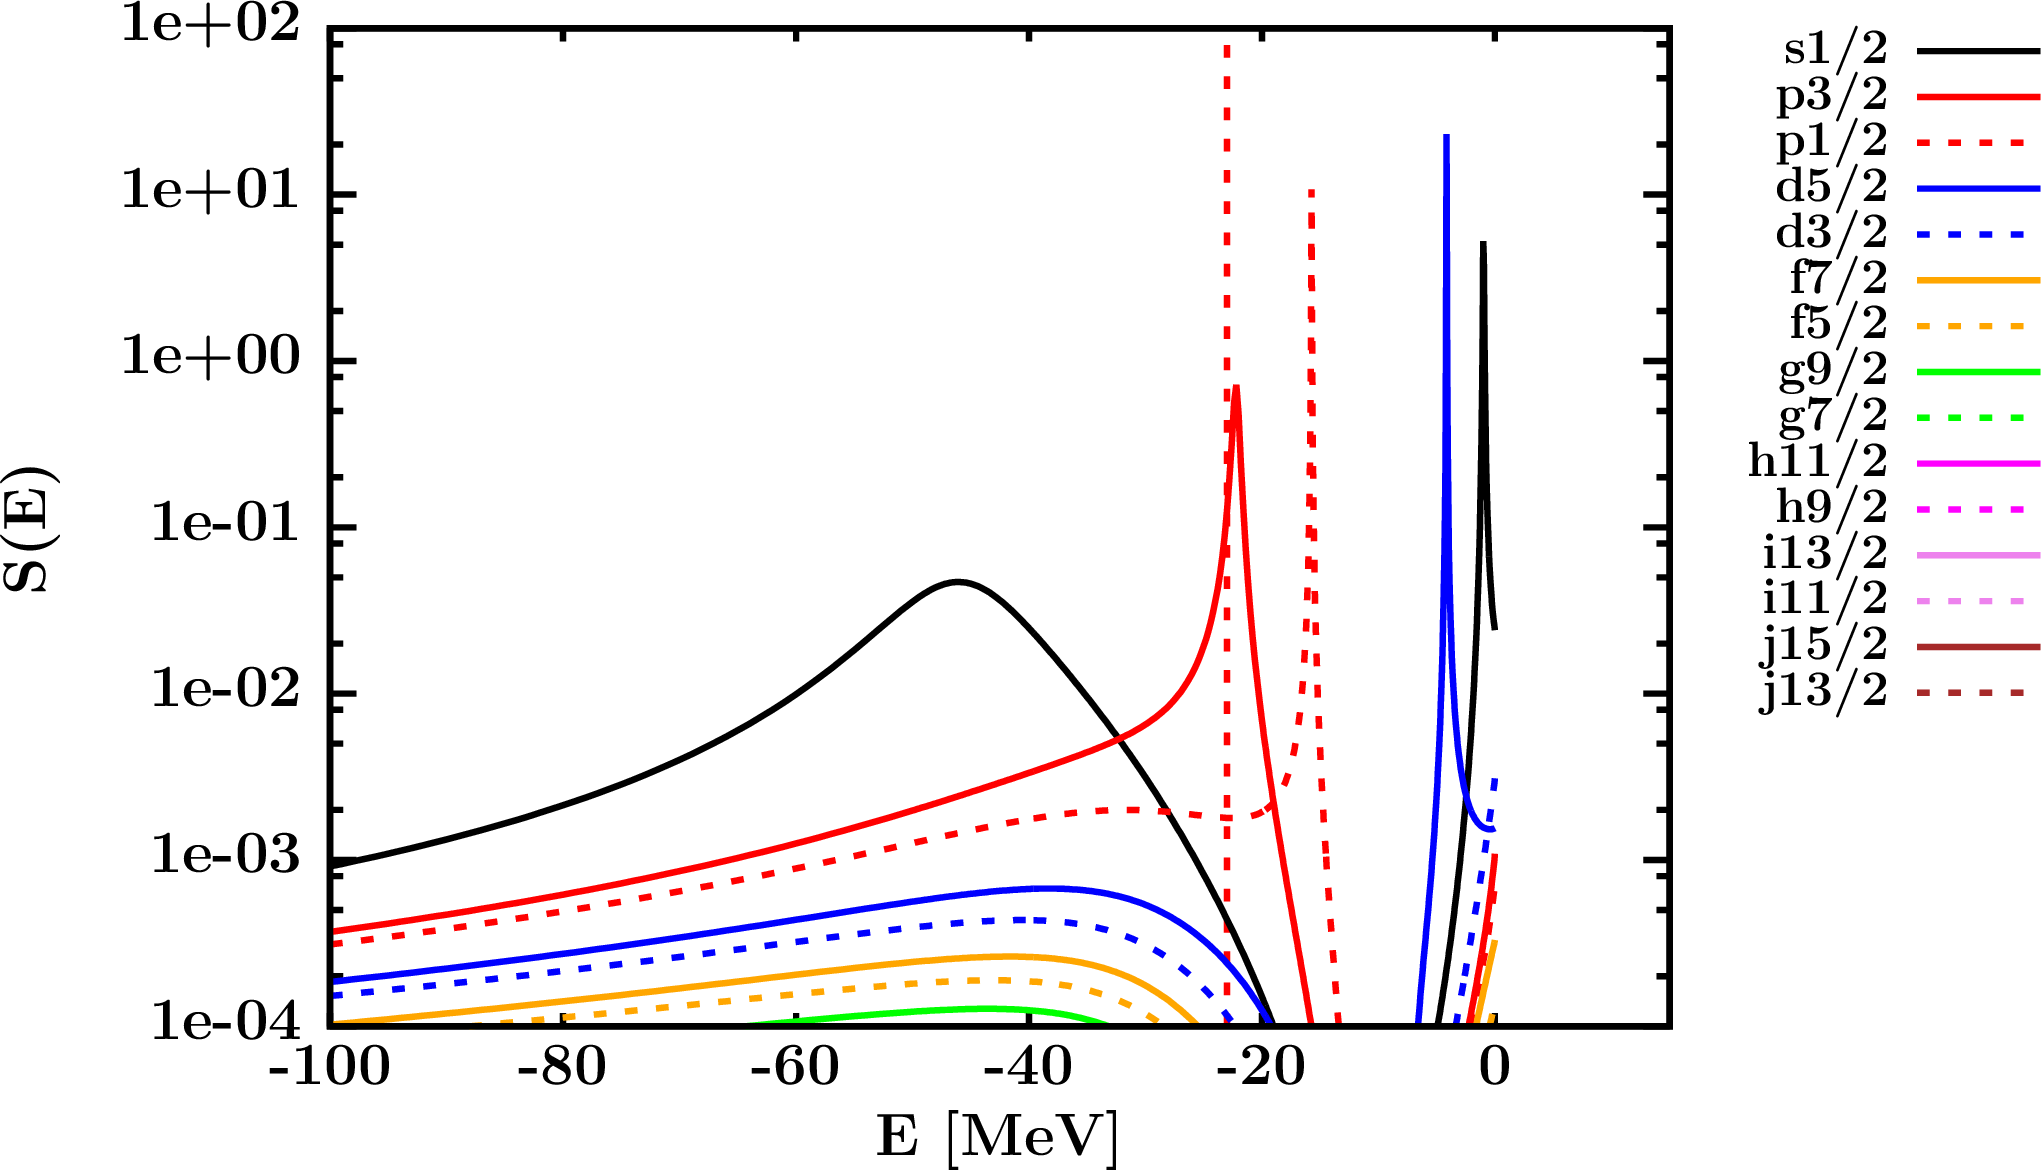
\includegraphics[width = 0.9\textwidth]{figures/o16_neutronSpectralFunctions.png}
\caption{DOM calculation of $^{16}O$ neutron spectral functions}
\label{o16NeutronSpectralFunctions}
\end{center}
\end{figure}

\begin{figure}
\begin{center}
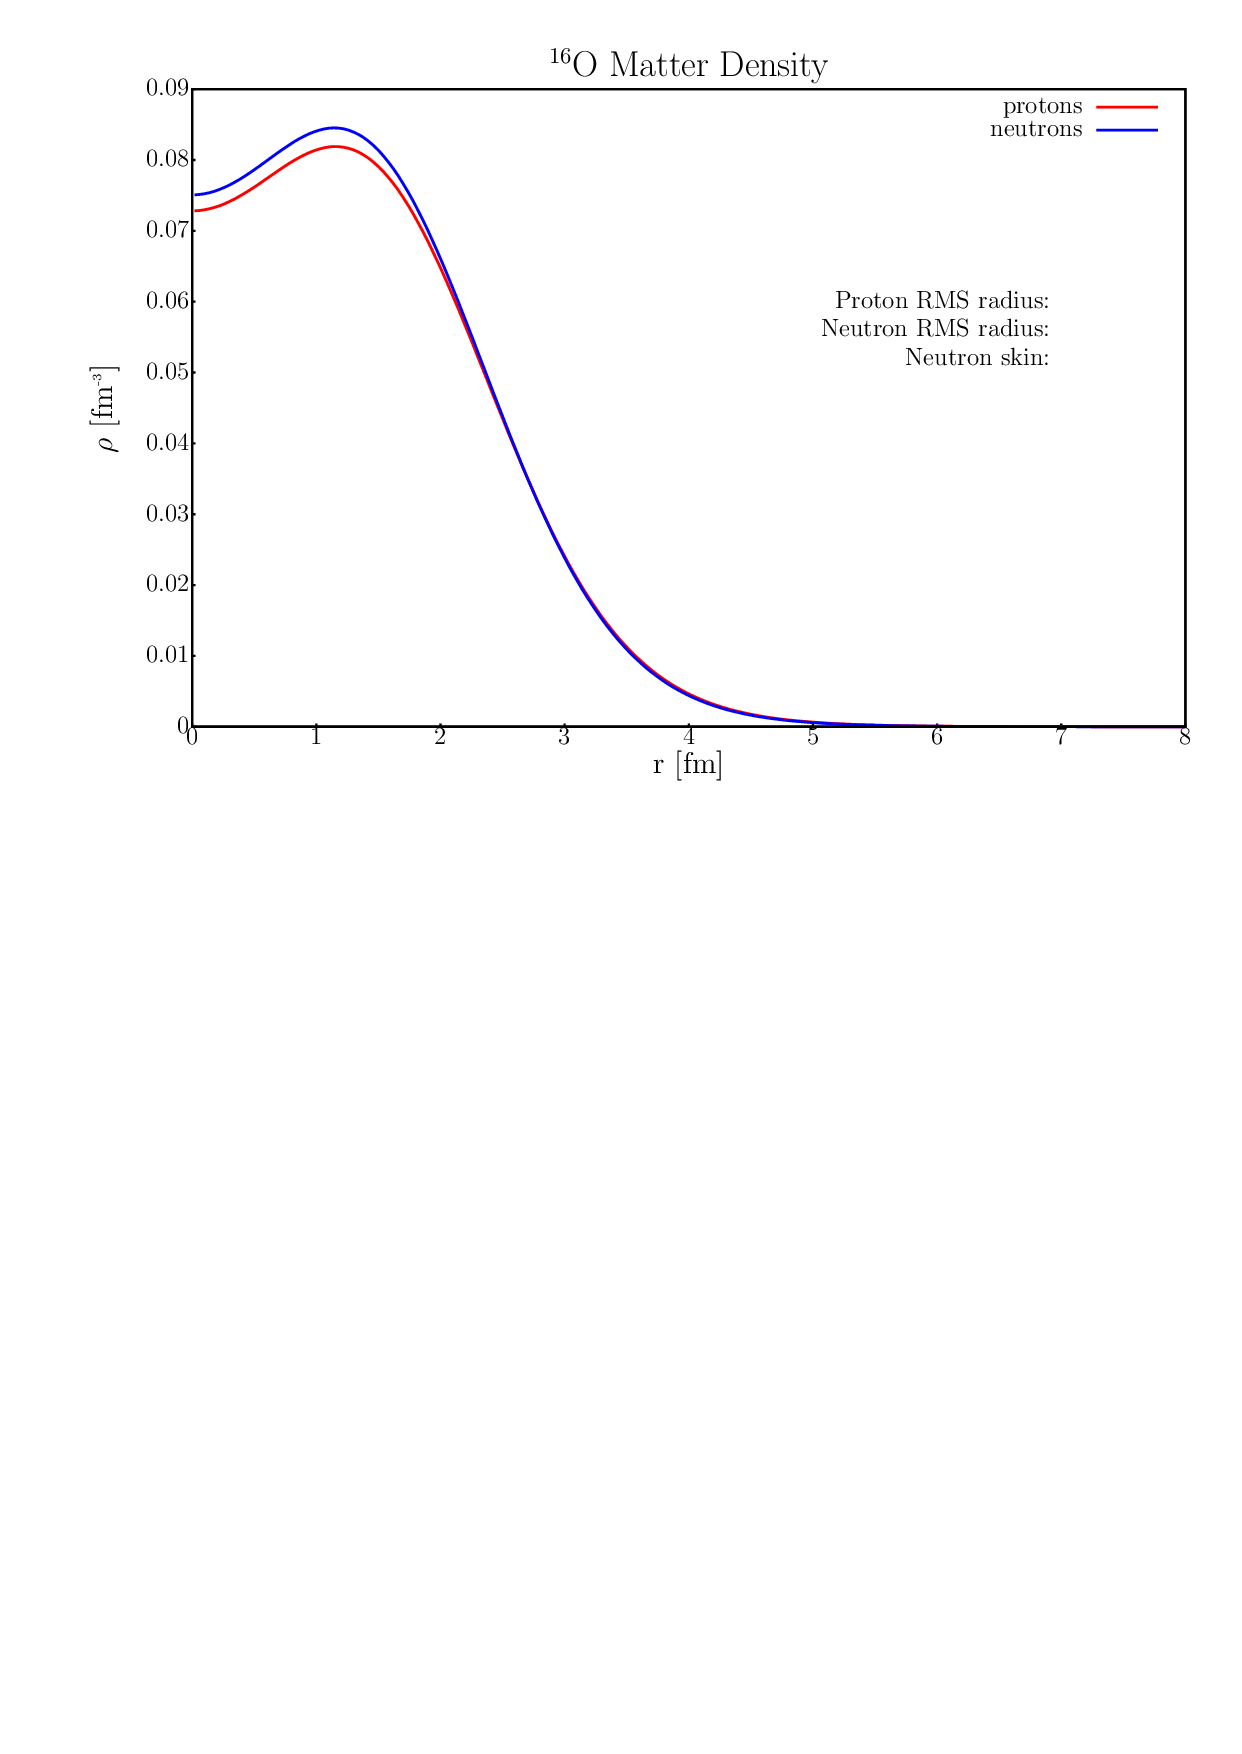
\includegraphics[width = 0.9\textwidth]{figures/o16_matterDensity.png}
\caption{DOM prediction of $^{16}O$ matter density}
\label{o16MatterDensity}
\end{center}
\end{figure}

%\begin{table}
%  \begin{center}
%    \caption{Calibration beams and the energies generated with the degraders.}\label{CBeams}
%  \begin{tabular}{ccccc}
%    \hline \hline
%    Species & Energy & Target & Thickness & Degraded Energy  \\ 
%            & [MeV/A] & &[mg/cm$^2$] & [MeV/A] \\
%     \hline
%    $p$ & 24.2 &  Au & 20.0 & 24.0   \\
%           &  & Al & 429 & 15.8 \\
%    \hline
%    $d$ & 24.2 &  Au &20.0 & 24.1 \\
%            & & Al & 429 &20.3 \\
%    & &  Al & 858 & 15.8 \\
%            & 12.0 &  Au & 20.0 & 11.9 \\
%    \hline
%    $\alpha$ & 24.0 &  Au & 20.0 & 23.8 \\
%     & & Al & 429 &15.6 \\
%    \hline \hline
%  \end{tabular}
%\end{center}
%\end{table}

\afterpage{\clearpage}
